% 2010 年四川卷理科第 15 题：二面角 α-l-β，AB⊂α，B∈l，AB 与 l 成 30°。
% 来源 PDF：普通高考/2010/2010四川理.pdf，SHA-256 499425696359cfc2cf4418254bdaa1a37487b3dbaa072ff3c7cbe18dbabe73dc。
% 原页：第 1 页（A3 三栏）第 3 栏上部，书页码 631。
% 重绘依据：l 为水平棱，α 在其上方（左侧展开）、β 在其下方（右侧展开），两面沿 l 铰接；
%   A 在 α 内，自棱上一点 B 连到 A。
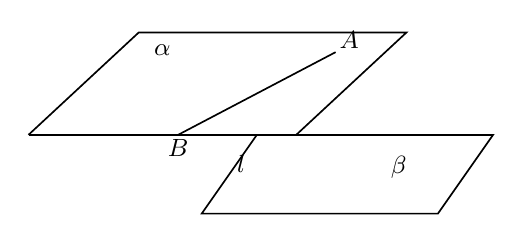
\begin{tikzpicture}[semithick, every node/.style={inner sep=1.2pt, font=\small}]
  % 棱 l
  \draw (-3.00,0) -- (2.90,0);
  % 平面 α（上方）
  \draw (-3.00,0) -- (-1.60,1.30) -- (1.80,1.30) -- (0.40,0);
  % 平面 β（下方）
  \draw (-0.10,0) -- (2.90,0) -- (2.20,-1.00) -- (-0.80,-1.00) -- cycle;
  % AB
  \coordinate (B) at (-1.10,0);
  \coordinate (A) at (0.90,1.05);
  \draw (B) -- (A);
  % 标注
  \node[below] at (-0.30,-0.20) {$l$};
  \node[below] at (B) {$B$};
  \node[above right] at (A) {$A$};
  \node[above] at (-1.30,0.95) {$\alpha$};
  \node[below right] at (1.55,-0.22) {$\beta$};
\end{tikzpicture}
